\section{Safety and Incident Contributors}
In NLR Air Transport Safety Institute's (an embedded research and consultancy organization within the Non-profit organisation 'National Aerospace Laboratory' in Netherlands, an institute which European Aviation Safety Agency (EASA) uses data from) report, "Aircraft ground handling and human factors" finished in April 2010, on the; "... causal factors which lead to human errors during the ground handling process and create unsafe situations, personal accidents or incidents." (Page 1 of the report); it was found that the largest safety related issues according to operational personnel and management comes from standardization of phraseology on the ramp and human factors such as time pressure, stress, fatigue and communication. This part of the report will describe the detailed findings of the query related to this project and their recommendations to the ground handling companies.

\subsection{Incidents}
First of all, one of the interesting findings, in the report, was that of what types of accidents happen, and at what relative frequency. In figure \ref{FrequencyOfIncidents}, we can clearly see that incidents that cause operational disruptions, equipment damage and aircraft damage happen at least once a week. As described in section [Freight] damage will not only be costly to repair, it will also most likely cause airplane delays, which can be very expensive for the airlines. Of course operational disrupts also result in delays and therefore loss of income.

\begin{figure}[H]
\centering
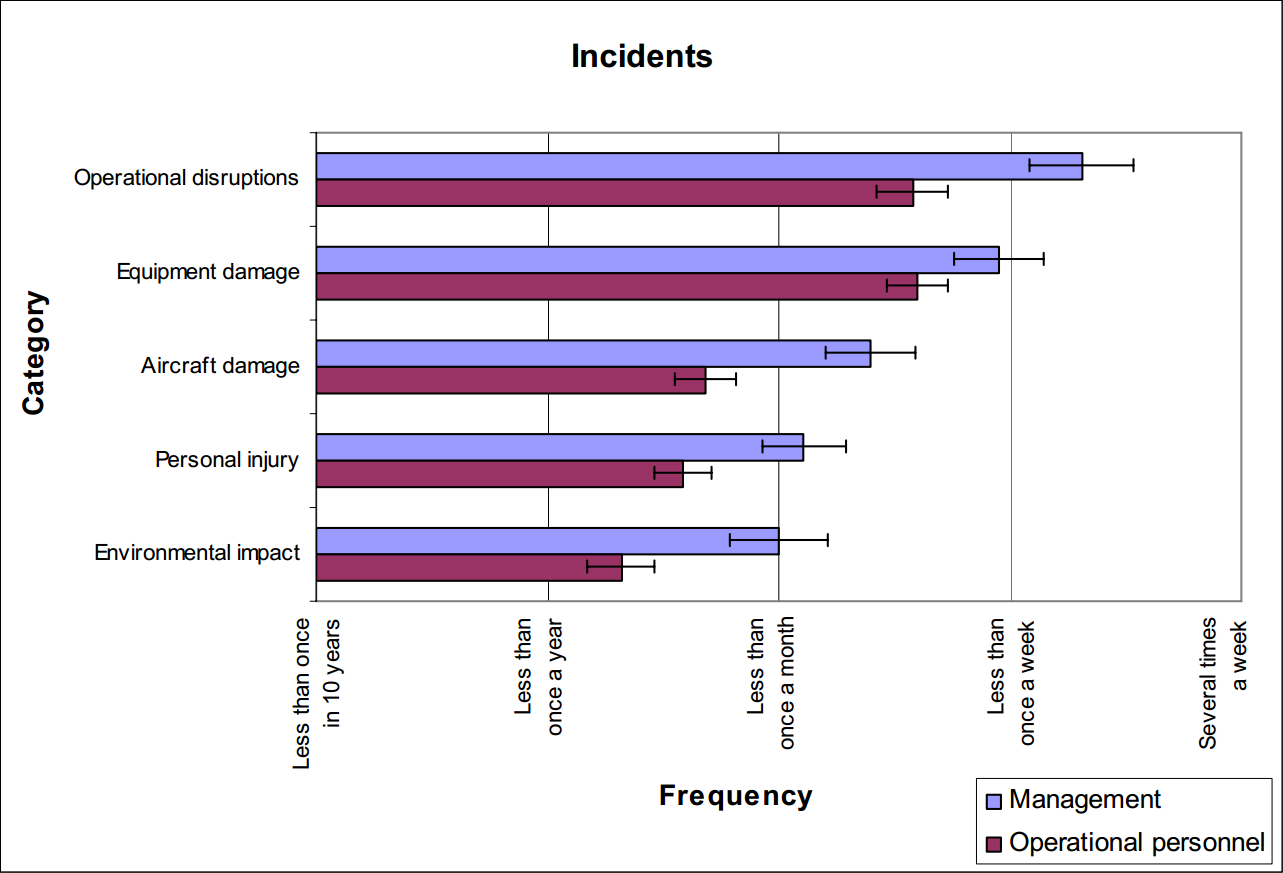
\includegraphics[width=\textwidth]{Grafik/FrequencyOfIncidents}
\caption{The frequency of how often incidents of different categories happens.}
\label{FrequencyOfIncidents}
\end{figure}

To underline this point the study found that delay of incoming and departing flights as a cause of these incidents each happens around once a week (page 29).

\subsection{Contributing factors} %IMP
Furthermore the survey also researched the contributing factors and how often they contribute to the different kind of accidents. As seen i figure \ref{ContributingFactors} it was found that the two most contributing factors are personal and communication, i.e. mistakes made by people and errors in the communication between people.

\begin{figure}[H]
\centering
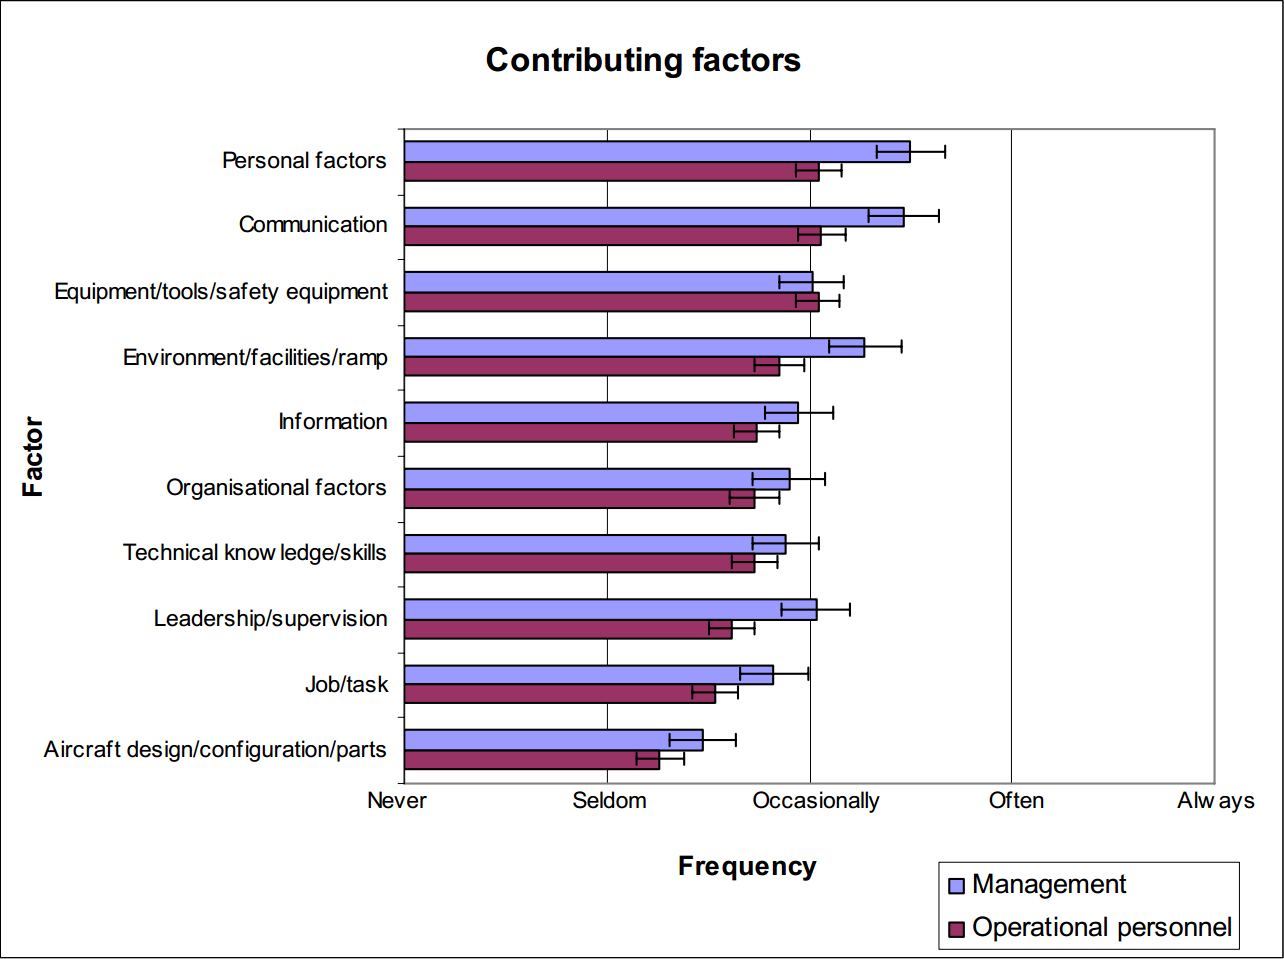
\includegraphics[width=\textwidth]{Grafik/ContributingFactors}
\caption{The contributing factors and how often they contribute to accidents.}
\label{ContributingFactors}
\end{figure}

Next to these two factors Environment/facilities/ramp and Leadership/supervision also receive a high rating from the two groups. 

\subsection{Personal Factors} %IMP
A very important conclusion, related to our project, in the report is which factors contribute to personal errors and mistakes made by operational personnel and management. As seen in figure \ref{PersonalFactors} it was found that the three major factors contributing to errors and mistakes made by the personnel is time pressure, stress, fatigue and also, very relevant to our project, motivation has a high rating. Especially time pressure is a very high contributor according both operational personnel and management, also because it is expected that both stress and fatigue most likely is a consequence of time pressure. In interviews made with both management and the operational personnel it was found that the reason for fatigue is most likely caused by the ground handling staff having to work double shifts (for different employers) to generate sufficient income. Also these interviews expressed that professional pride to meet the departure time may result in shortcuts have to be taken.

\begin{figure}[H]
\centering
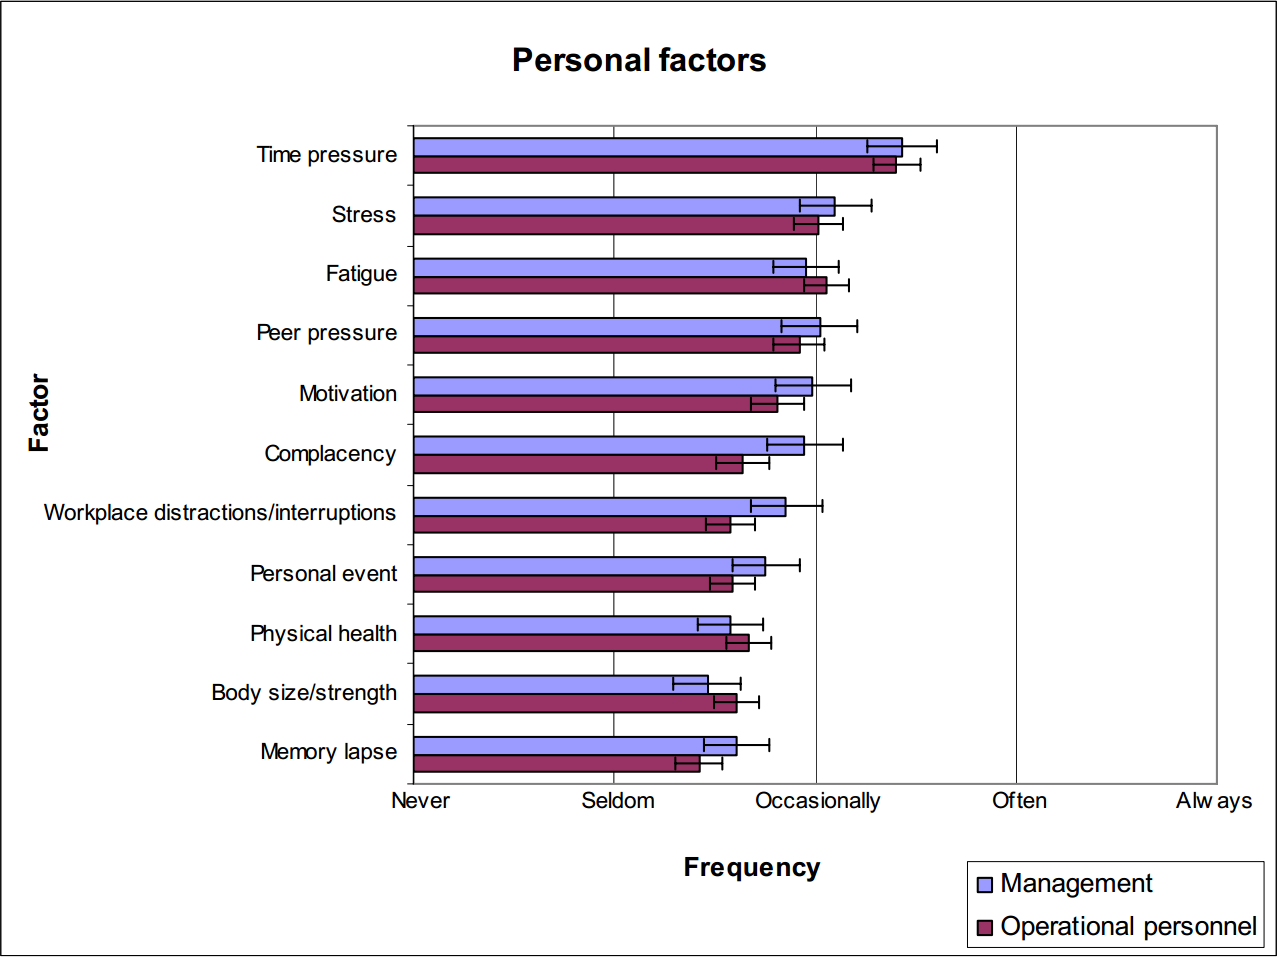
\includegraphics[width=\textwidth]{Grafik/PersonalFactors}
\caption{Breakdown of channels used to book flights.}
\label{PersonalFactors}
\end{figure}

Therefore it is very important to take these contributors into account when considering a solution to prevent and solve the problem which is damage to aircraft, equipment, personal injury, operational disrupts and environmental impact.

\subsection{Safety}
When considering safety it is important to consider weather to work safely or to meet the scheduled departure time is prioritized highest by the employees. In one of the interviewers it was expressed that it is often thought that the quicker and better the personnel is meet the departure times the more unsafe the work gets, but in reality there is always a balance and if that balance is met safety is not compromised.

\subsection{Communication}
The communication of safety issues is considered important for the personnel to learn from each other and take proactive action. It is therefore considered important to have a safety reporting system and actually both management and operational personnel did not know or recognize any reporting system in their own ground handling organization.

\begin{figure}[H]
\centering
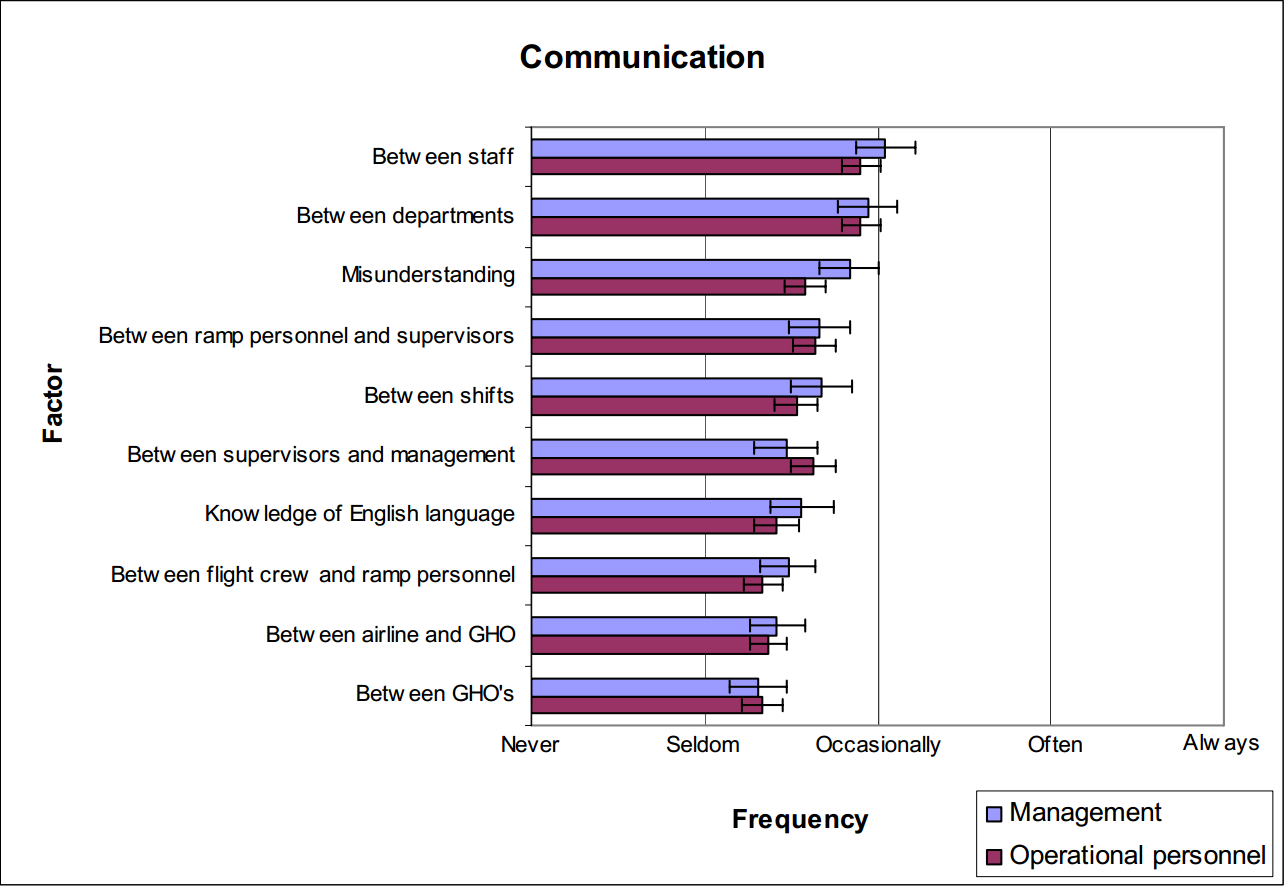
\includegraphics[width=\textwidth]{Grafik/CommunicationalFactors}
\caption{What kind of miscommunication causes incidents and errors.}
\label{CommunicationalFactors}
\end{figure}

\subsection{Environment}
According to the survey both management and the operational personnel agree that, when talking about factors surrounding the environment, facilities and ramp, which is the forth highest contributor, rain, wind and snow is the highest contributors. Also humidity, cold and lightning is high contributors. This means that the inefficiency and the rate of accidents, errors and incidents is significantly higher if the weather is bad.

\subsection{Information} %IMP
The fifth highest contributor is information, as seen in figure \ref{Information} most information errors contribute nearly similar except  incorrect manufacturer/aircraft documentation which is the lowest contributor. This is most likely caused by the fact that ground handling personnel is not closely associated with these documents since their company documents already have the procedures and manuals explaining the same.

\begin{figure}[H]
\centering
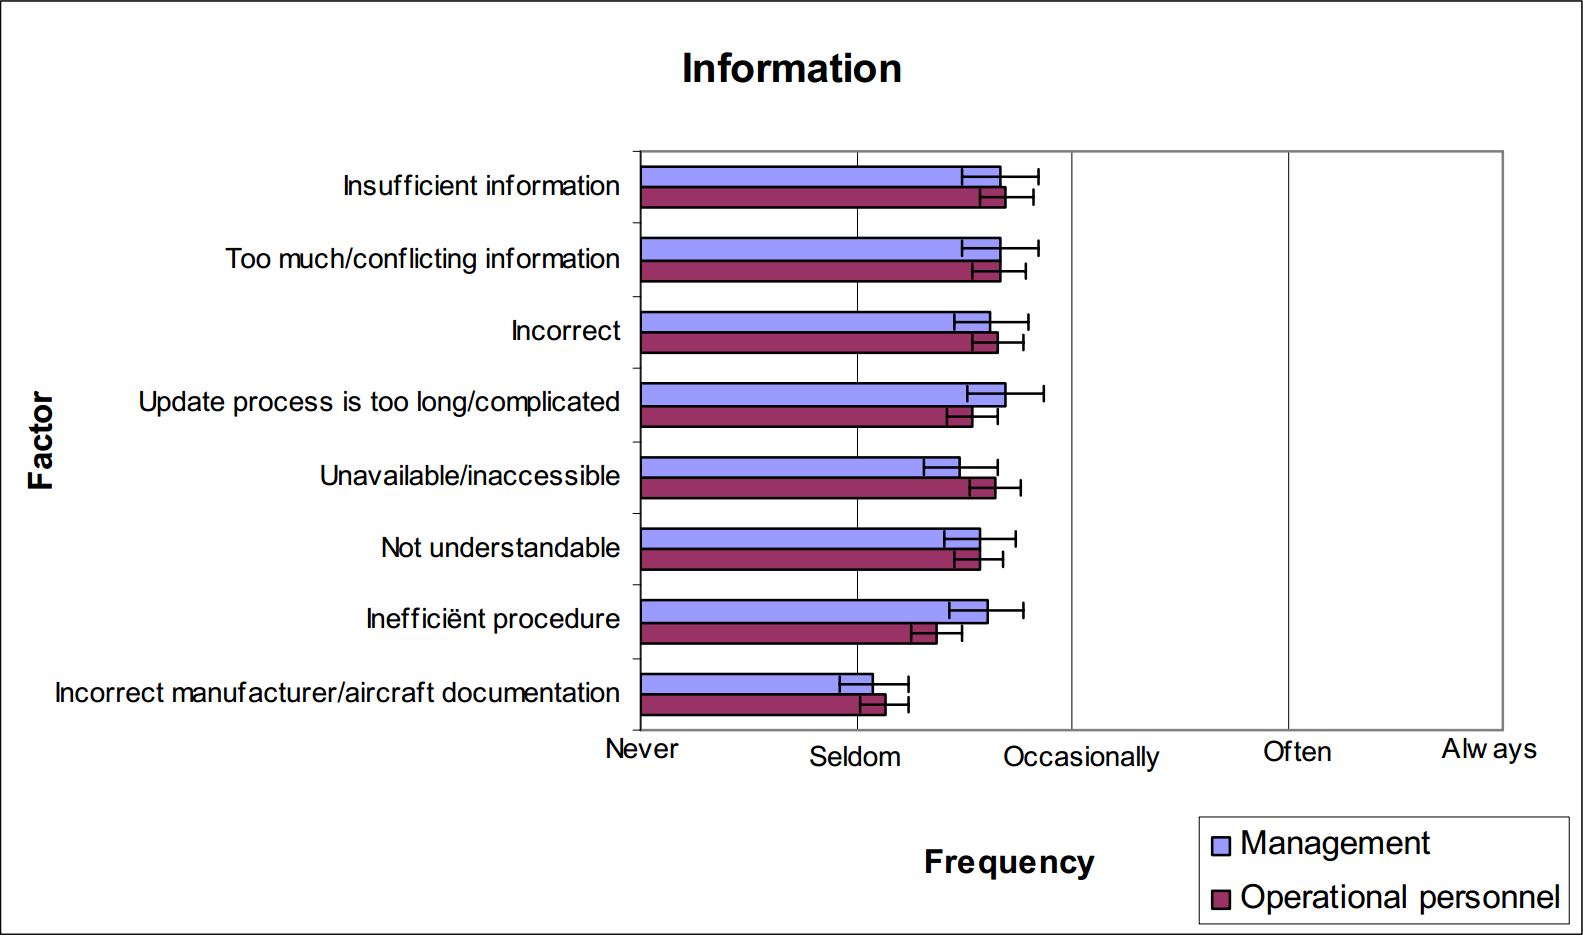
\includegraphics[width=\textwidth]{Grafik/Information}
\caption{Contributors to errors made because of incorrect information.}
\label{Information}
\end{figure}

It is important though to keep in mind that communication can only be effective if the information is correct and these things therefore need to be in order.

\subsection{Management} %IMP
Considering organizational factors moth Management and Operational personnel agrees the insufficient personnel is the biggest contributor, though this is express significantly stronger by the operational personnel. In the interviews made with both groups it was expressed that given the current economic tense climate, turnarounds are scheduled with a minimum amount of personnel. This of cause mean that delay and incidents are harder to deal with and therefore more experienced personnel is needed.

\begin{figure}[H]
\centering
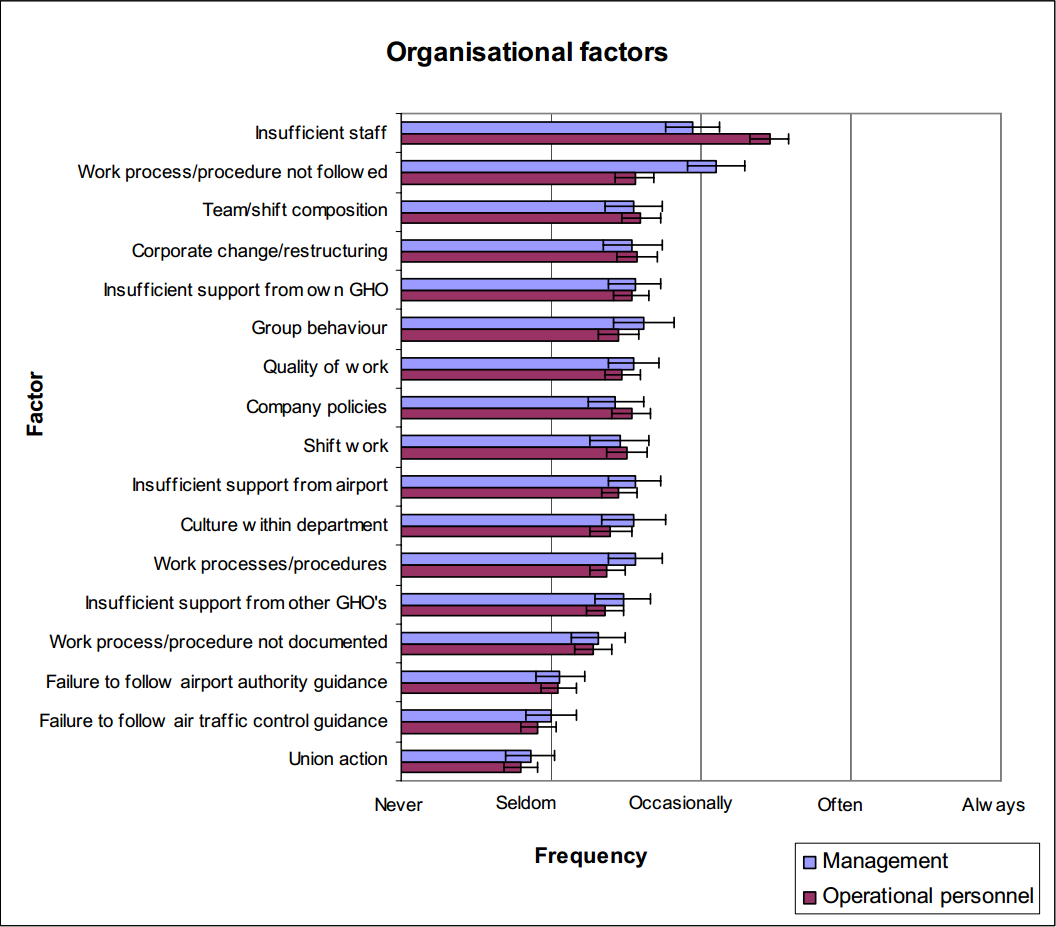
\includegraphics[width=\textwidth]{Grafik/OrganisationalFactors}
\caption{Contributors to bad organization.}
\label{OrganisationalFactors}
\end{figure}

\subsection{Technical factors}
In figure \ref{TechnicalFactors} the important thing is to note that the highest contributor to errors and incidents is task planning. Therefore it is important that the planning of the personnel tasks and also skills is done properly to avoid errors and incidents.

\begin{figure}[H]
\centering
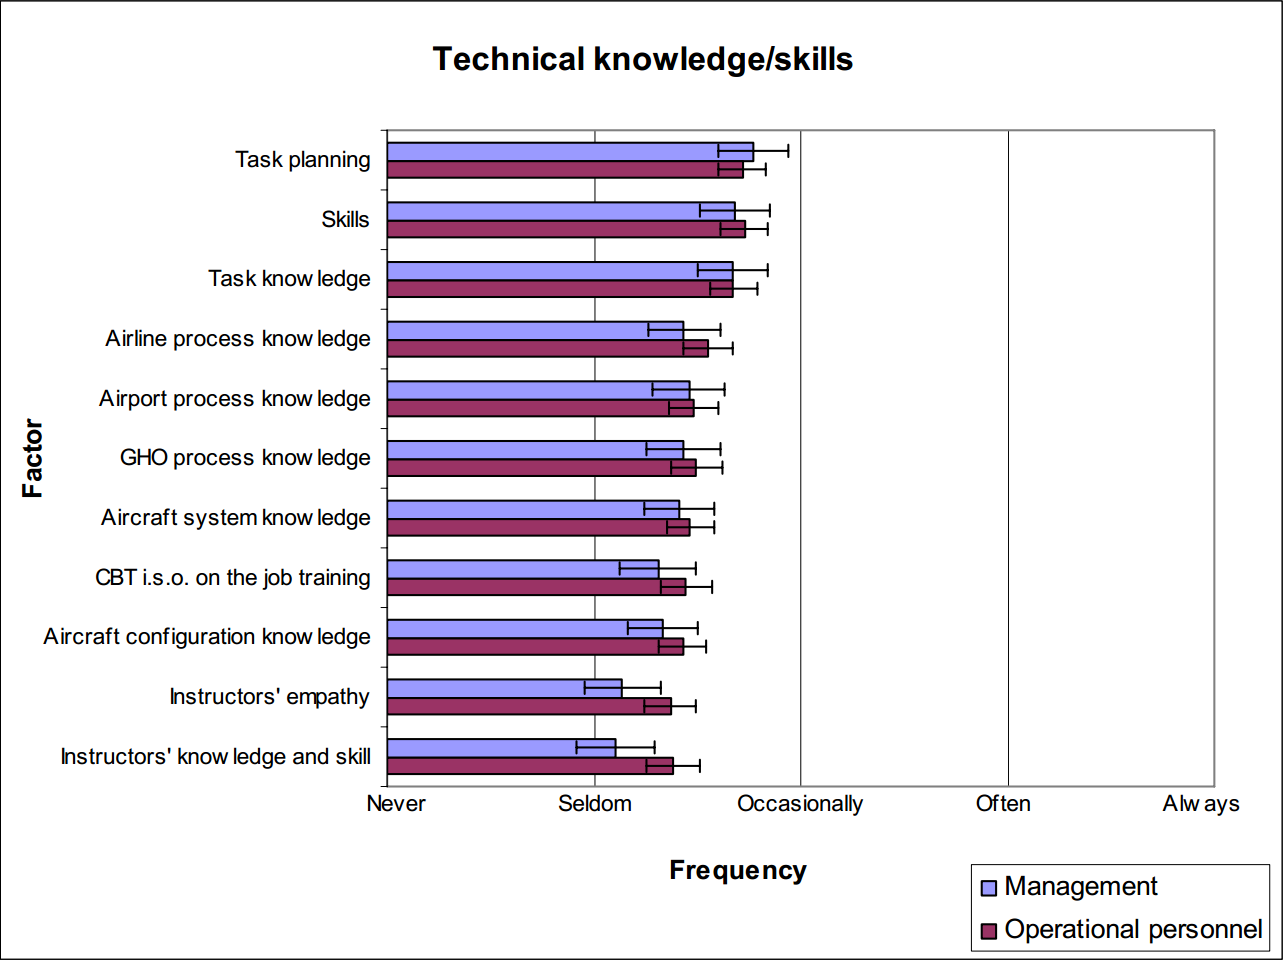
\includegraphics[width=\textwidth]{Grafik/TechnicalFactors}
\caption{Technical contributors to errors and incidents.}
\label{TechnicalFactors}
\end{figure}

\subsection{Leadership}
The Study also shows that the biggest contributors when talking about leadership, which is the 8th largest contributor to errors, is motivation, prioritization of work and planning. This shows that, when trying to remove the problem discussed in the section, motivating and organizing the workday is very important.